\chapter{Commands used in Estimation and Simulation}

\chapauthor{Stephen P. Hughes}{NASA/Goddard Space Flight Center}
\chapauthor{Darrel J. Conway}{Thinking Systems, Inc.}
\chapauthor{Matthew P. Wilkins}{Schafer Corporation}

GMAT's Solver subsystem uses a finite state machine model to drive the algorithms implanted in the solvers.  Each Solver object implements its own state machine, and pairs that state machine with a command or set of commands that manipulates GMAT's objects to provide data required for the algorithm.  The interaction between the solver and the command subsystem necessitates knowledge on the command side about the state information in the finite state machine.  In essence, the Solver finite state machine drives both the solver algorithm and a paired state machine implemented in the corresponding command.  The state and state transitions of the solution process is always controlled in the Solver object.  Object manipulations are performed in GMAT's Mission Control Sequence -- and in particular, in the Solver Control Sequence that uses the Solver object.

Each type of Solver is matched to command.  The targeters, like the differential corrector, are paired with the Target/EndTarget commands, and use the Vary and Achieve commands for additional communications needed by the targeting algorithms.  The optimizers are paired with GMAT's Optimize/EndOptimize commands, and use the Vary, Minimize, and NonlinearConstraint commands for communications.

There are four commands designed to pair with the estimation solvers: RunEstimator, RunSimulator, and (in the future) an Estimate/EndEstimate subsequence pair and a Simulate/EndSimulate subsequence pair.  This document describes the state machine activities for the first two commands. The subsequence based command pairs are not part of the first release of GMAT's estimation capabilities, and will be designed (along with any communications related commands) at a later date.

\section{Command Usage in GMAT}

Missions in GMAT are always executed by executing commands in a Mission Control Sequence.  The Mission Control Sequence is a linked list of command objects.  It is executed inside of one of GMAT's Sandboxes starting with the first node in the list, and progressing until the end of the list is executed.  The Sandbox drives this process when GMAT's Moderator calls the Sandbox's Execute() method.  The Sandbox tracks the executing command using a current command pointer, initially set to the first command in the list.

When the mission is run, the Sandbox checks for user interrupts, and then calls the Execute() method
on the current command pointer, executing that command.  Upon return from this call, the Sandbox
updates the current command pointer by calling the command's GetNext() method.  The pointer returned
from this call is then checked; if it is NULL, the Mission Control Sequence has run to completion.
If the returned pointer is not NULL, it points to the next command that needs to be executed, and
the process repeats by checking for interrupts and then calling the Execute() method on the command
pointed to by the current command pointer.  Thus overall control of the process running in GMAT's
Sandbox is managed by the commands in the Mission Control Sequence.

Some of the commands in the Mission Control Sequence manage their pointers to the next command in a reentrant fashion.  All of the commands that manage subsequences -- GMAT's ``branch commands'' -- work this way, as do the commands like Propagate that might take a long time to execute.  The call to GetNext() for these commands can return a pointer back to the command itself, rather than the next command in the list.  This self reference in the list transversal call (i.e. the call to ``GetNext()'') lets GMAT perform other processing during execution of time consuming commands.

\section{Estimation Command Overview}

\begin{figure}[htbp]
\begin{center}
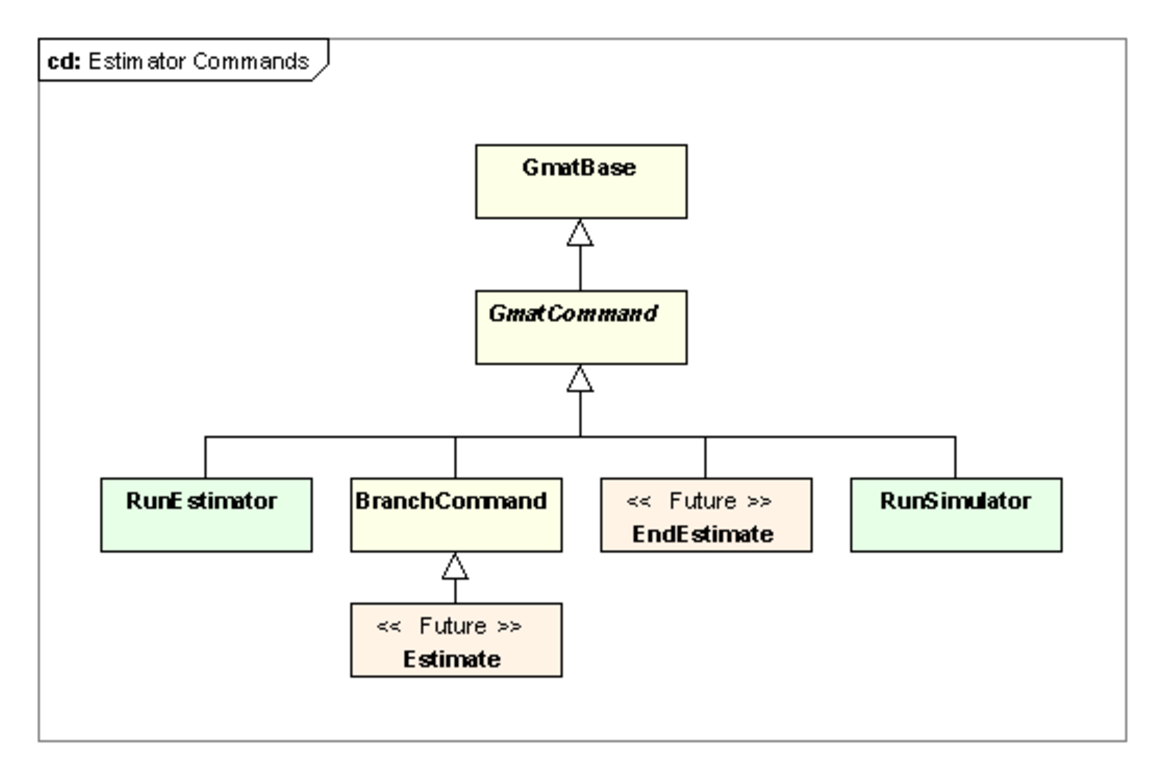
\includegraphics[scale=0.6]{Images/EstimatorCommands.eps}
\caption{\label{fig:EstimatorCommands}Commands Used in Estimation}
\end{center}
\end{figure}

The three command sets used for estimation -- RunEstimator, RunSimulator, Estimate/EndEstimate, and Simulate/EndSimulate, shown in Figure~\ref{fig:EstimatorCommands} -- all follow a similar methodology at the level of command execution. The commands interact with the estimator and simulator components to run the solver's finite state machine.  Each solver implements a state machine tailored to the needs of the implemented algorithm.

At the highest level, the state machine executes at prompting from the command, which in turn was prompted by a call from the Sandbox containing the Mission Control Sequence, as is shown in Figure~\ref{fig:EstimatorCommandCallSeq}. The estimation command is part of the Mission Control Sequence assigned to a Sandbox in GMAT.  When GMAT runs the Mission Control Sequence, it checks for user interrupts, and then calls the Execute method in the current command in the Mission Control Sequence.  The figure shows the high level flow that occurs for this process when the current command pointer is an estimation command, including the interactions between the command and the estimator.

\begin{figure}[htb]
\begin{center}
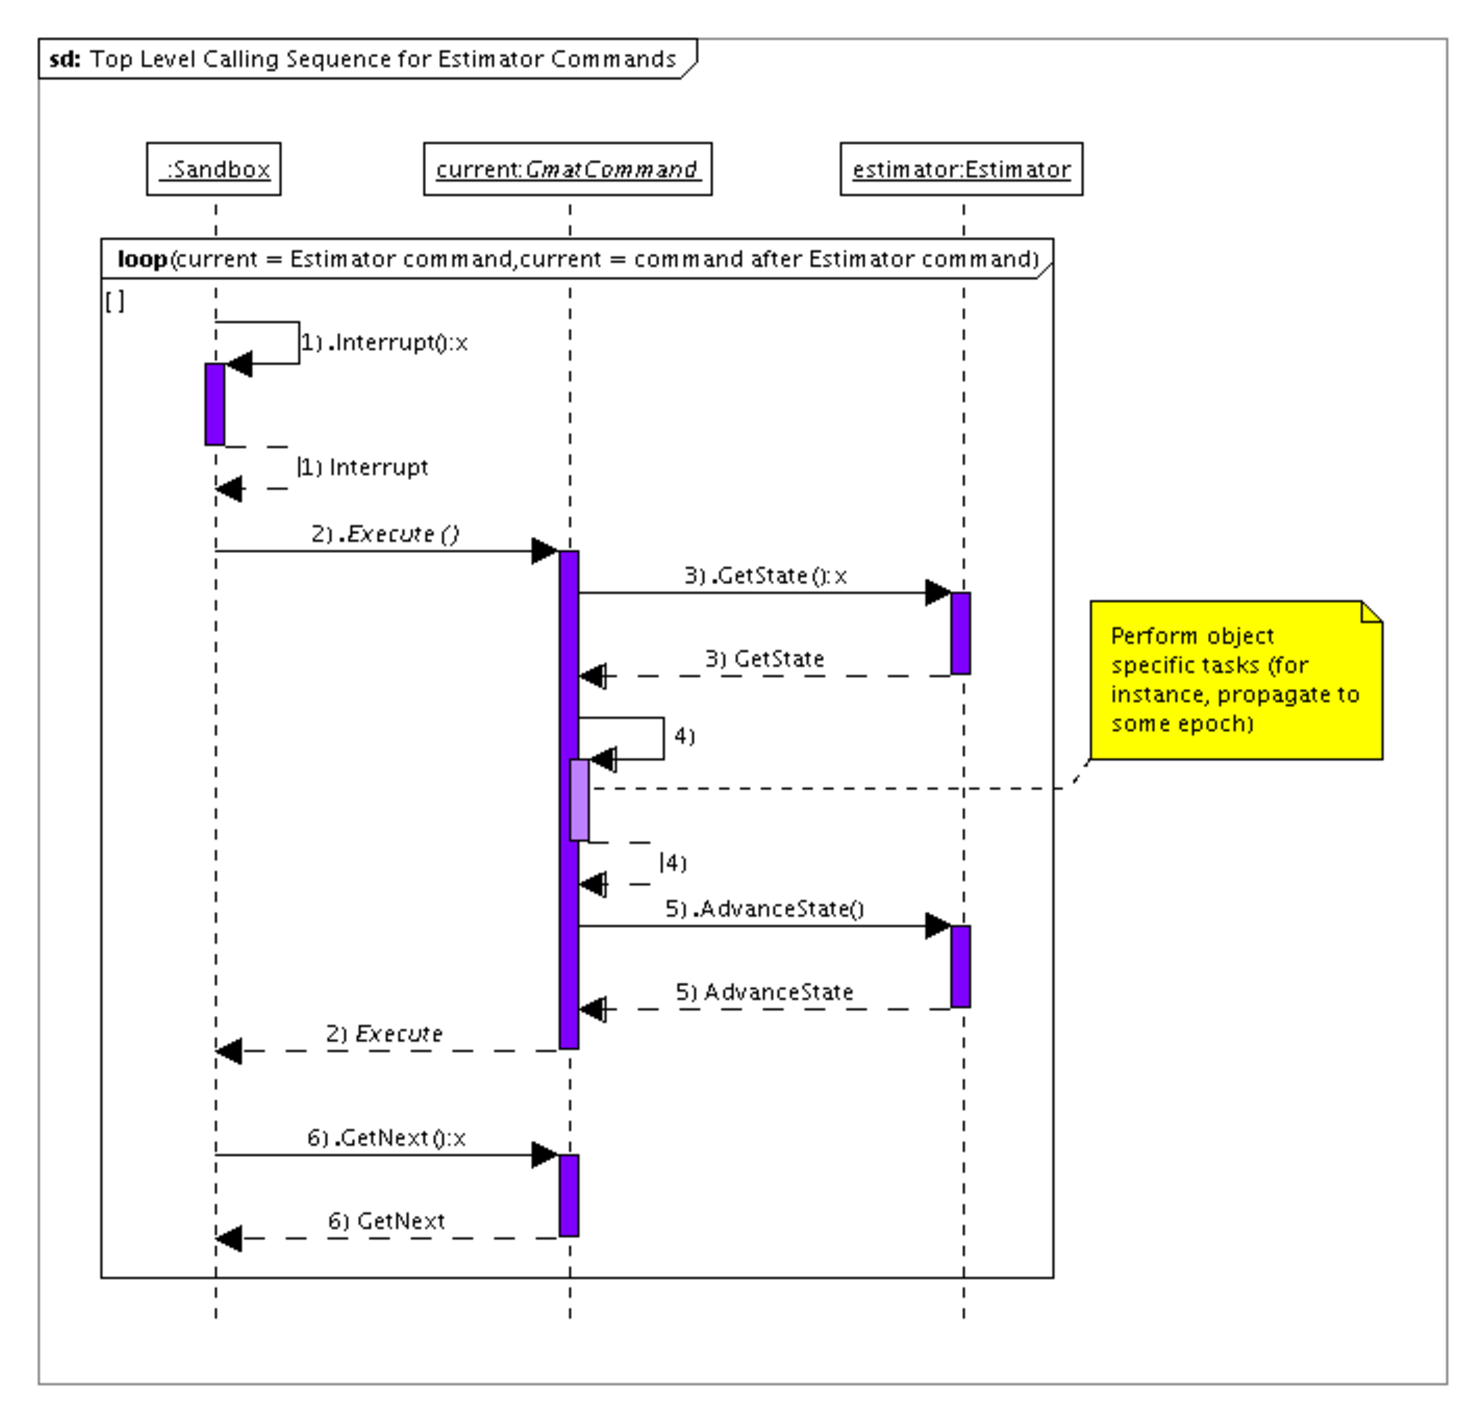
\includegraphics[scale=0.5]{Images/TopLevelCallingSequenceforEstimatorCommands.eps}
\caption{\label{fig:EstimatorCommandCallSeq}Top Level View of State Machine Execution}
\end{center}
\end{figure}

Each time the estimator command receives a call from the Sandbox to execute (made via the Execute() method), it queries the estimator for the current state, performs any requisite command actions based on that state, and then calls AdvanceState() on the solver so that the solver can perform the next action dictated by the state machine.  Upon return from the call to AdvanceState(), the command returns control to the Sandbox, which checks for user interrupts, and then calls the command's GetNext() method to determine the next command that needs to be executed.  The estimation command returns its pointer from this call as long as the solver's state machine is running.  The Execute() method is called on the command, which lets the estimation command process the next state in the state machine.  This sequence repeats until the estimation state machine runs the actions required by the FINISHED state, completing the estimation process.  Once the process has completed, a subsequent call to the command's Execute() method returns a reference to the next command in the Sandbox's Mission Control Sequence.

This general framework for estimation command execution in GMAT follows the basic execution framework for all GMAT commands: the Sandbox checks for interrupts, then executes the command, then retrieves the pointer to the next command to execute, and continues this process until the Mission Control Sequence is finished running.

This overview is intended to provide a framework for understanding the details of how the Estimation commands work in GMAT.  The following sections describe the estimation commands using the Batch Least Squares estimator to show the state machine elements of the design.  The state machine itself is described in the batch estimator section of this document.  The interactions required on the command side for the batch and sequential process are identical; from the point of view of the command, the process is to take an action, call AdvanceState() on the estimator, and repeat until the estimator reports that the process is complete.  We'll begin by examining the RunEstimator command.

\section{The RunEstimator Command}

The RunEstimator command drives the estimation process when the evolution of the participants can be modeled through propagation from one epoch to the next.  RunEstimator is a propagation-enabled command, meaning that it includes methods and data structures needed to perform propagation.  It supplies methods for performing actions in estimator state machines that support the following states:

\begin{itemize}
\item INITIALIZING
\item PROPAGATING
\item LOCATING
\item CALCULATING
\item ESTIMATING
\item CHECKINGRUN
\item FINISHED
\end{itemize}

The RunEstimator command provides methods that are called when the estimator's state machine is in one of these states and the Execute() command is called.  (The command's initialization is performed prior to the state machine call that detects the INITIALIZING state, so there is no need for a machine command function for that call.)  The command methods that perform actions based on the state of the estimator's state machine are listed here, and described in the command method description below.

\begin{itemize}
\item \textbf{INITIALIZING}:  Calls the PropagateToStart() method
\item \textbf{PROPAGATING}:  Calls to the Propagate() method
\item \textbf{LOCATING}:  Calls the PropToEvent() method
\item \textbf{CALCULATING}:  Calls the Calculate() method
\item \textbf{ESTIMATING}:  Calls the Estimate() method
\item \textbf{CHECKINGRUN}:  Calls the CheckConvergence() method
\item \textbf{FINISHED}:  Calls the Finalize() method
\end{itemize}

Different estimators can use different states in their state machines, and are likely to use the states in a different order based on the estimation algorithm.  For example, the batch least squares estimator does not use the ESTIMATING state until after all of the tracking data has been processed, while the sequential filters like the extended Kalman filter will estimate -- that is, advance through the ESTIMATING state -- as the data is processed.

Figure~\ref{fig:RunEstimatorStateMachine} shows the finite state machine for the batch least squares estimator (the lower portion of the sequence partition) and the RunEstimator command.  The core interaction supplied by the command during execution of the state machine for this example is the propagation of the participants in the estimation process.  The batch estimator performs the other steps of the estimation process without need for direct interaction with the command.

\begin{figure}[htb]
\begin{center}
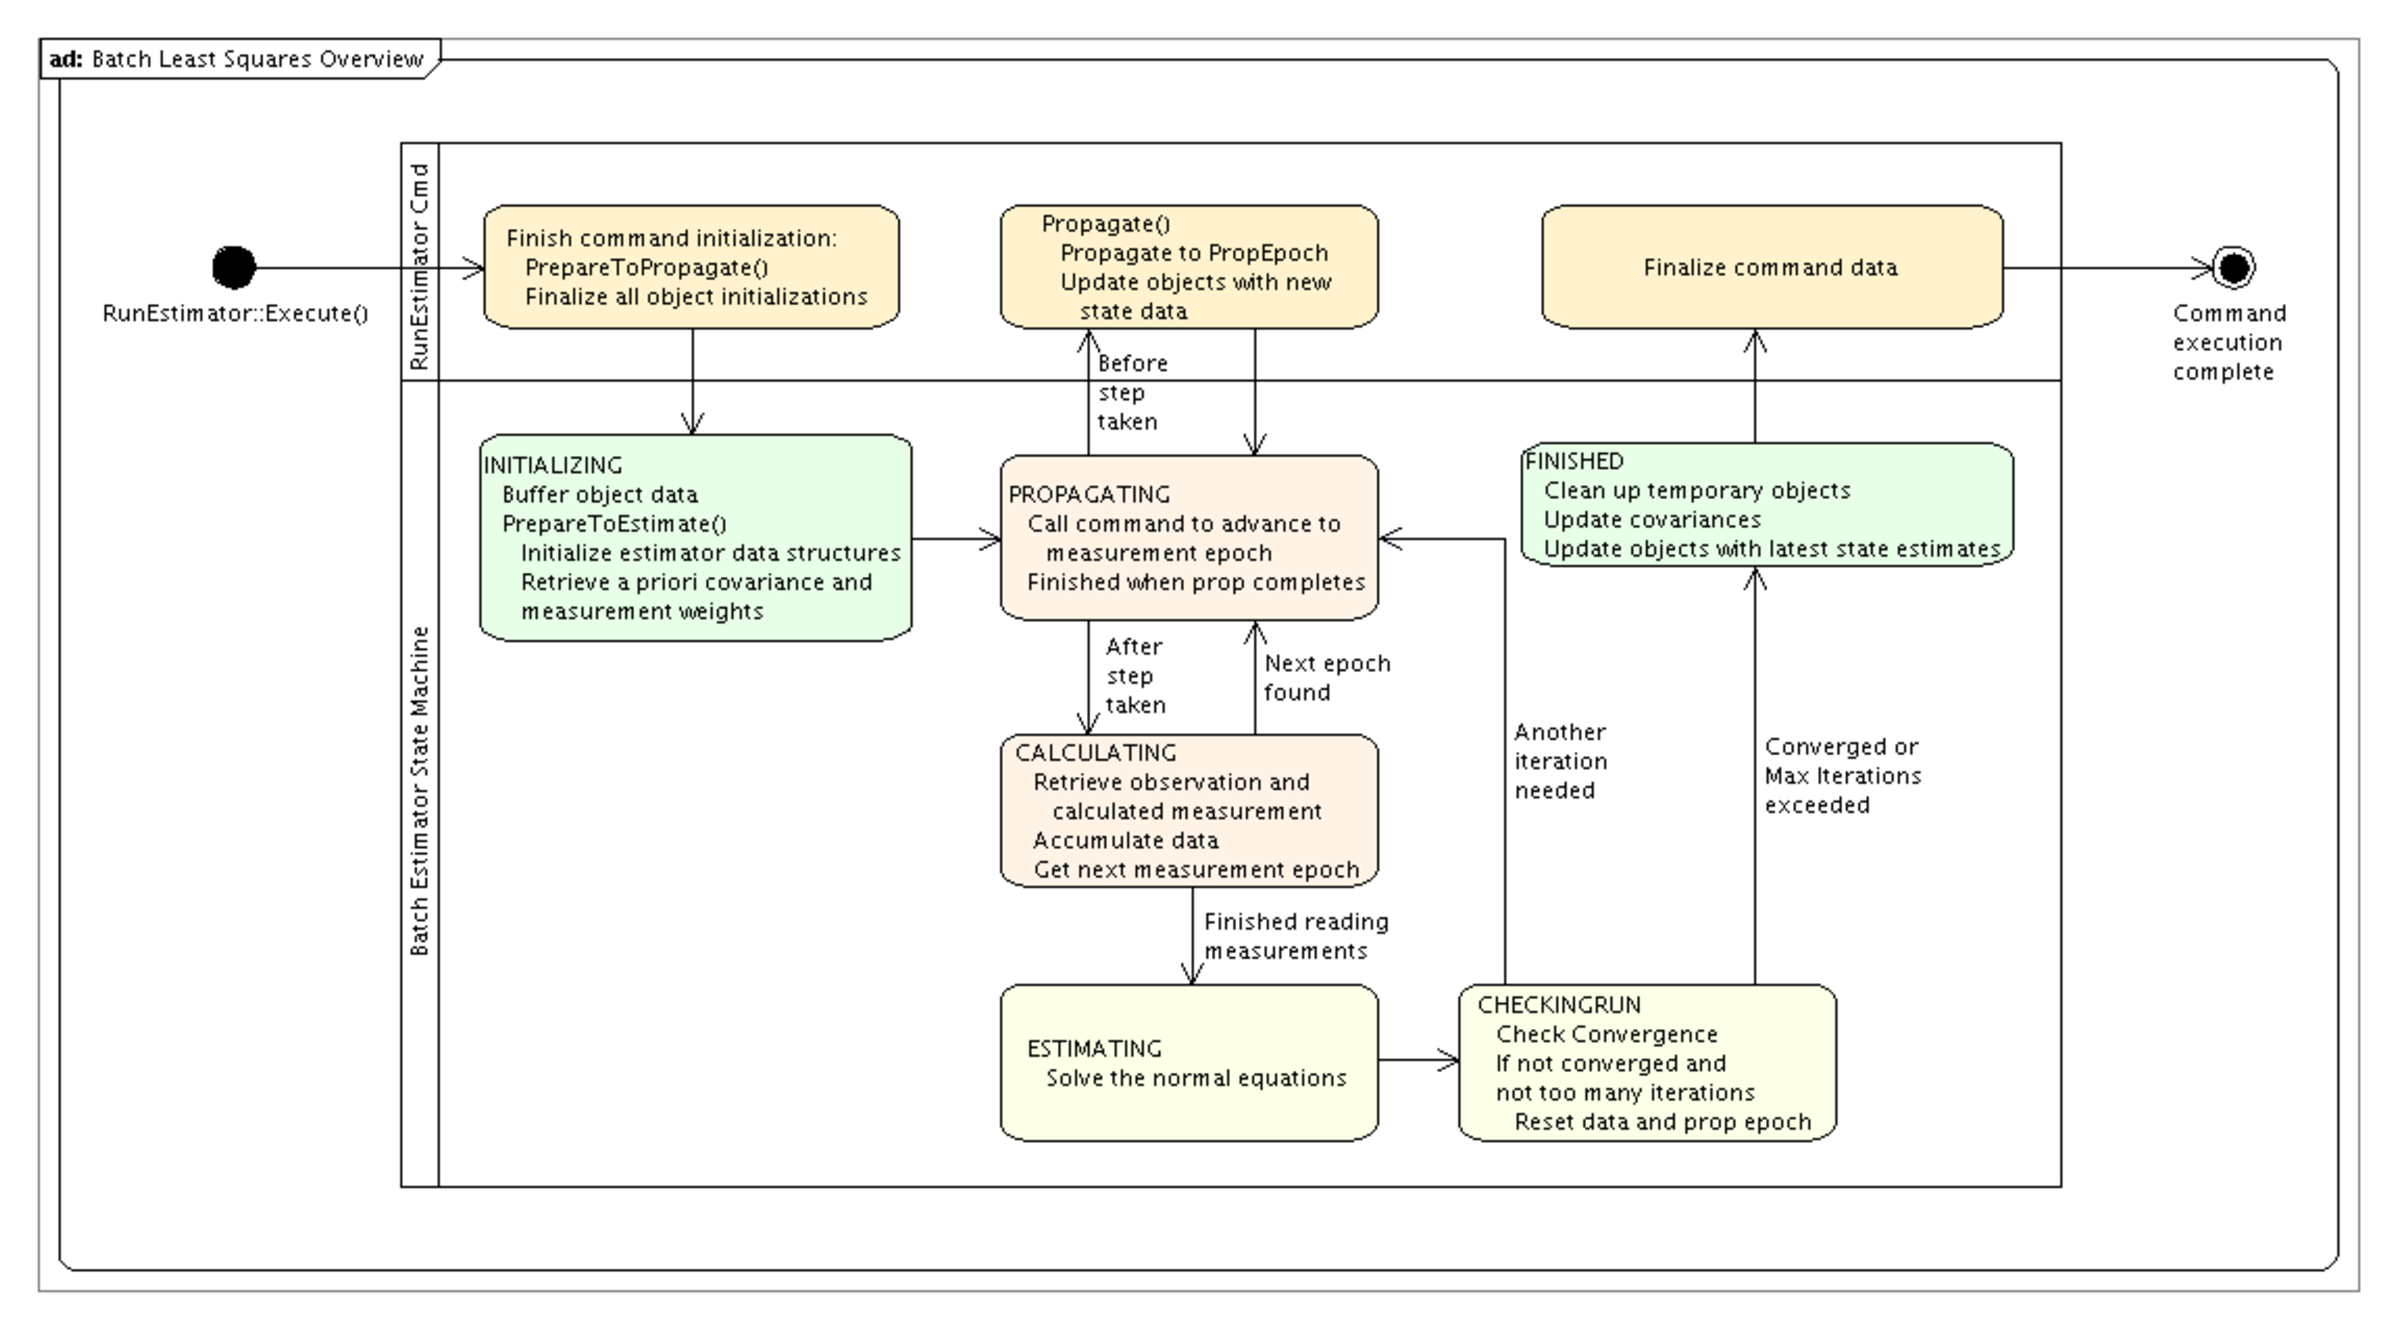
\includegraphics[scale=0.4]{Images/BatchLeastSquaresOverview.eps}
% BatchLeastSquaresOverview.png: 1134x621 pixel, 72dpi, 40.01x21.91 cm, bb=0 0 1134 621
\caption{\label{fig:RunEstimatorStateMachine}Interactions Between the RunEstimator Command and the Batch Least Squares Estimator}
\end{center}
\end{figure}

Three of the states specified here require propagation from the command.  The INITIALIZING state requires that the command perform propagation from the current state epoch to the estimation epoch specified on the estimator.  GMAT's objects are advanced from their current epoch to the next measurement epoch through calls to the Propagate() method, made when the finite state machine is in the PROPAGATING state.  Finally, event location to perform tasks like light-time corrections requires propagation.  These tasks are performed while the state machine is in the LOCATING state.

For each of these propagation steps, the RunEstimator command needs to know the size of the time step required to change from the current epoch to the desired epoch.  This information is retrieved from the estimator using the FindTimeStep() method.  The returned time step is then used to step the participants using a PropSetup reference in the command.  That reference, set during command initialization, points to the propagator owned by the estimator.  A future enhancement may allow the replacement of the estimator's propagator with a event-specific propagator tailored to the participants in the event calculation for propagation triggered from the LOCATING state.

The details of the state machine execution are described in the sections describing each specific estimator.  The description provided here is intended to specify the command actions required in the estimation process.

\subsection{RunEstimator Members}

The RunEstimator command contains the following data members and methods.

\paragraph{RunEstimator Attributes}

\begin{itemize}
\item \textbf{std::string estimatorName}:  The name of the Estimator that the command uses.
\item \textbf{Estimator *estimator}: A pointer to the Estimator.
\item \textbf{PropSetup *propagator}:  A pointer to the Propagator owned by the Estimator.
\end{itemize}

\paragraph{RunEstimator Methods}

\begin{itemize}
\item \textbf{virtual bool Initialize()}:  Sets internal references and interconnections, and prepares the estimator for use.
\item \textbf{virtual bool Execute()}:  Accesses the state from the finite state machine, performs any required command side actions, and then calls AdvanceState() on the estimator to move the finite state machine to its next state.
\item \textbf{virtual void PropagateToStart()}:  Queries the estimator for the time step required to propagate to the estimation epoch, and then performs that propagation.
\item \textbf{virtual void Propagate()}:  Queries the estimator for the next required time step, and then performs the required propagation.
\item \textbf{virtual void PropToEvent(bool restoreFromBuffer)}:  Queries the estimator for the time step estimated to find an event, and then performs the required propagation.  This method buffers the initial state data if restoreFromBuffer is false, and resets to that buffered data if restoreFromBuffer is true. A call to restore when the buffer has not been set results in an exception.
\item \textbf{virtual void Calculate()}:  Performs command side actions when the estimator is in the CALCULATING state.  This method is used to report intermediate data if the estimator text file is running in verbose mode.
\item \textbf{virtual void Estimate()}:  Performs command side actions when the estimator is in the ESTIMATING state.  This method is used to report intermediate data if the estimator text file is running in verbose mode.
\item \textbf{virtual void CheckConvergence()}:  Performs command side actions when the estimator is in the CHECKINGRUN state.  This method is used to report the status of the estimation process.
\item \textbf{virtual void Finalize()}:  Finalizes the command so that it can be reexecuted on a subsequent call. This method is also used to report the final estimated state and the status of the convergence criteria.
\end{itemize}

\section{The RunSimulator Command}

The RunSimulator command is a propagation-enabled command that manages the processes required to run and respond to the finite state machine defined in Simulator objects.  It supplies methods for performing actions in these state machines that when the finite state takes one of the following values:

\begin{itemize}
\item INITIALIZING
\item PROPAGATING
\item LOCATING
\item CALCULATING
\item SIMULATING
\item FINISHED
\end{itemize}

The RunSimulator command provides methods that are called when the simulator's state machine is in
one of these states and the Execute() command is called.  The command methods that perform actions
based on the state of the simulator's state machine are listed here, and described in the command
method description below.

\begin{itemize}
\item \textbf{INITIALIZING}:  Calls the PrepareToSimulate() method
\item \textbf{PROPAGATING}:  Calls to the Propagate() method
\item \textbf{LOCATING}:  Calls the PropToEvent() method
\item \textbf{CALCULATING}:  Calls the Calculate() method
\item \textbf{SIMULATING}:  Calls the Simulate() method
\item \textbf{FINISHED}:  Calls the Finalize() method
\end{itemize}

Figure~\ref{fig:RunSimulatorStateMachine} shows the finite state machine for the simulator in the lower portion of the sequence partition, and the non-trivial processes executed in the RunSimulator command.  The core interaction supplied by the command during execution of the simulator state machine is the propagation of the participants in the simulation process.  The simulator performs the other steps of the process without need for direct interaction with the command.

\begin{figure}[htbp]
\begin{center}
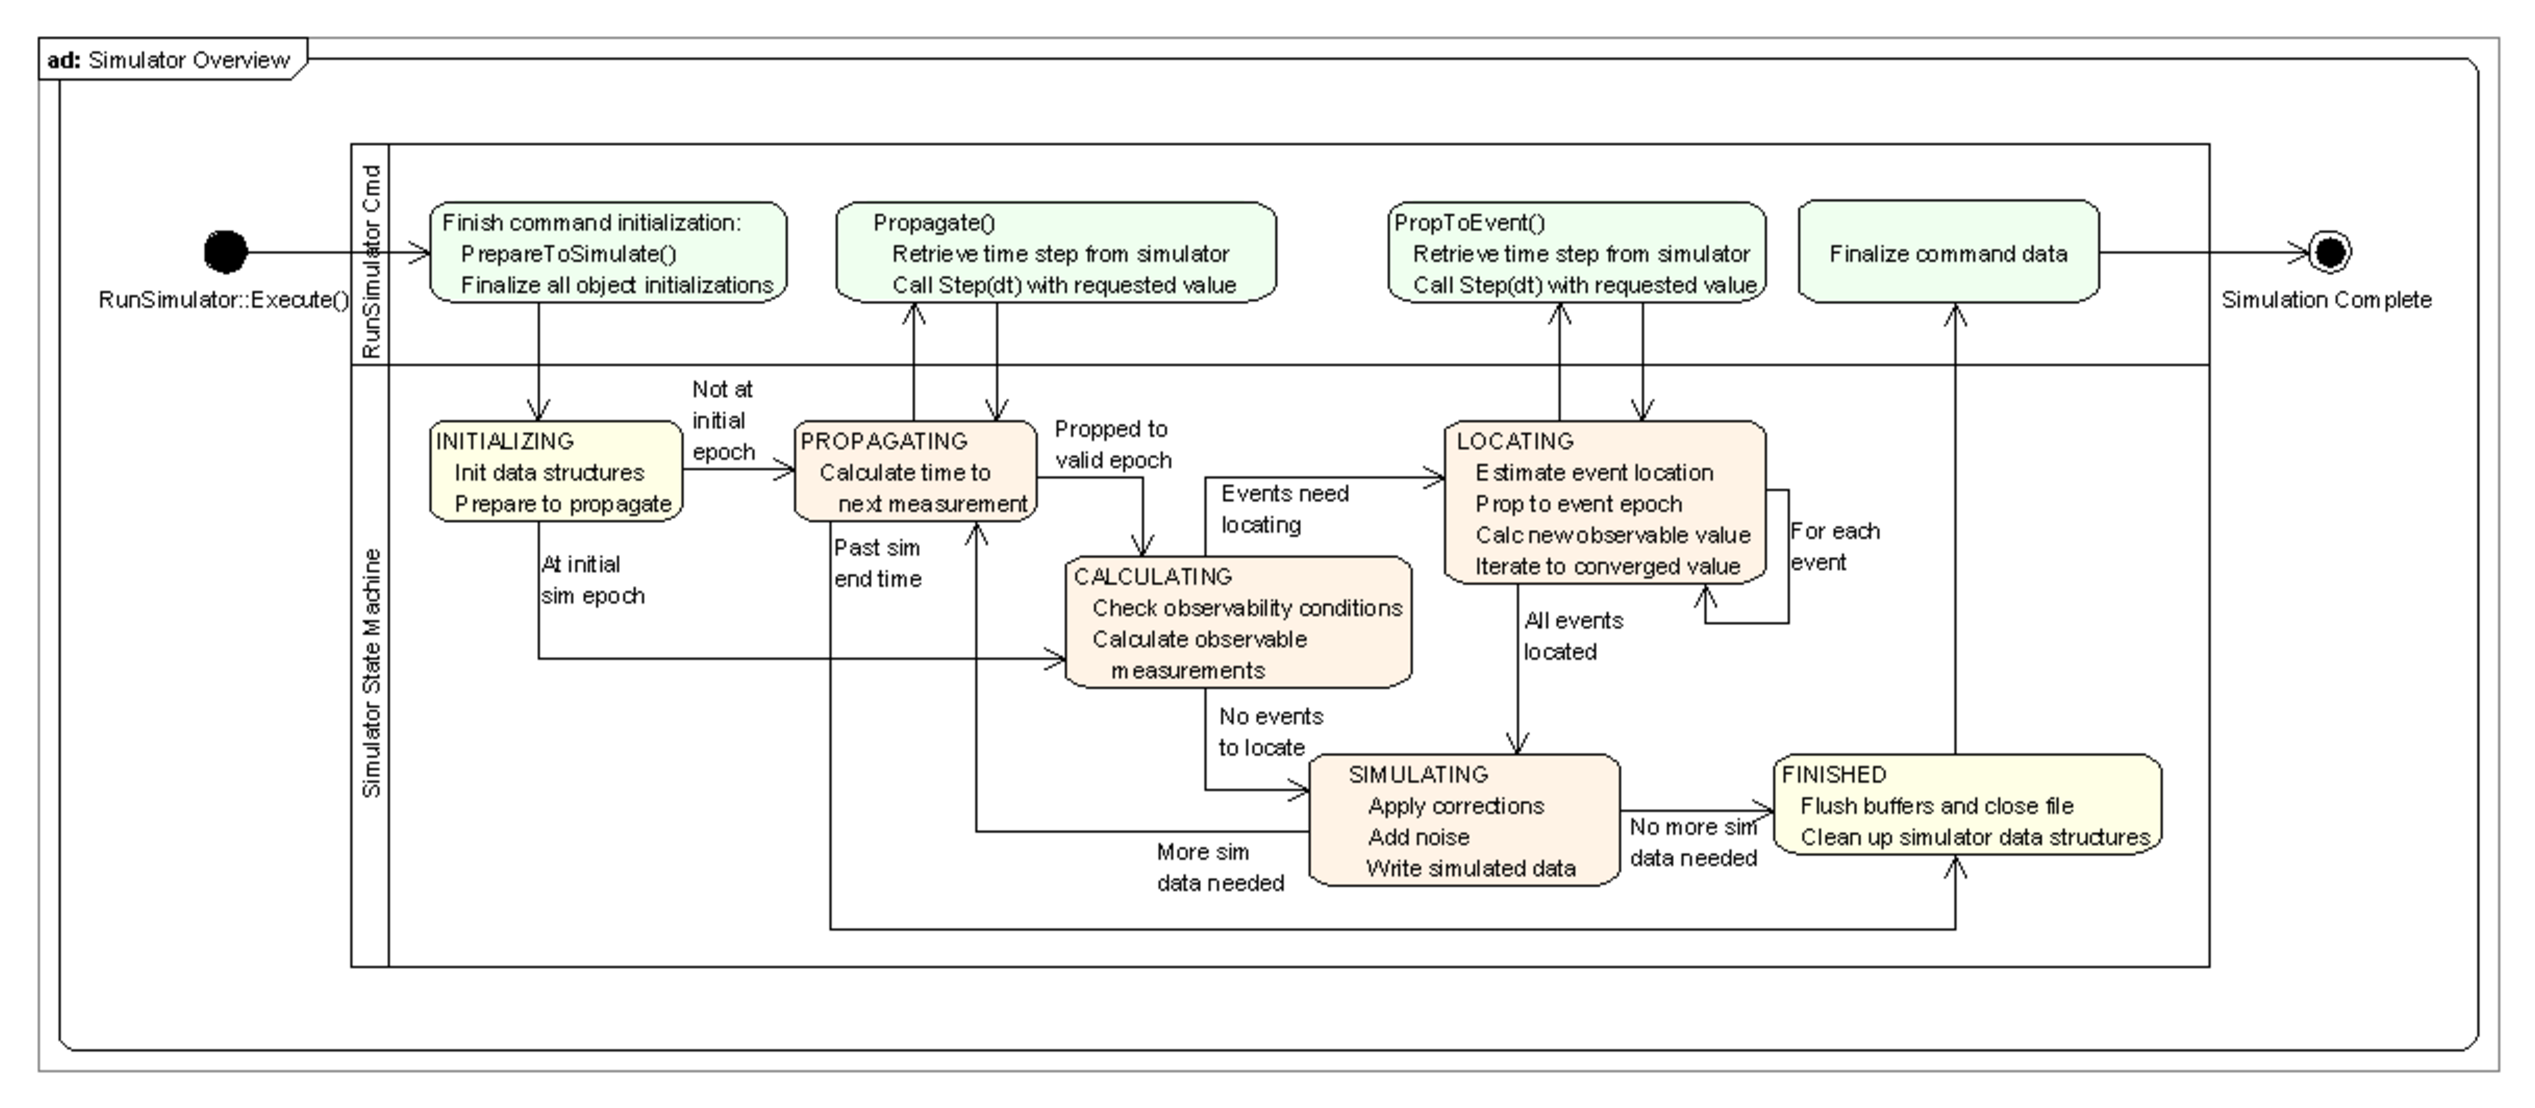
\includegraphics[scale=0.38]{Images/SimulatorOverview.eps}
% SimulatorOverview.png: 1201x516 pixel, 72dpi, 42.37x18.20 cm, bb=0 0 1201 516
\caption{\label{fig:RunSimulatorStateMachine}The Simulation State Machine}
\end{center}
\end{figure}

The RunSimulator command defines the interface between the Mission Control Sequence running in a Sandbox and a Simulator object.  The RunSimulator command manages all of the propagation performed in support of the simulation, simplifying the interrupt processing during the simulation.

In GMAT, the simulator object owns the propagator and the measurement manager.  The command retrieves the propagator pointer from the simulator for use during command execution.  The simulator also provides the information about the duration of any needed propagation to the command.  The RunSimulator command manages a buffer of objects that are propagated in support of the simulation, and uses this buffer to restore object data when performing calculations that would otherwise corrupt the time dependent states of those objects.  As an example, this object buffer is used during light time iterations so that the object states at the anchor time for a measurement can be restored after iteration has converged on the light time correction.

\subsection{Key Processes}

The RunSimulator command has two key processes, captured in the Initialize() and Execute() methods.

\subsubsection{Initialization}

The RunSimulator::Initialize() method performs the usual reference object location and setting tasks
performed by all commands.  For the RunSimulator command, this process involves finding the associated Simulator and cloning it for local use.  The Clone() process for a Simulator object includes a call that creates a clone of the propagator (a PropSetup object) used in the simulator.  The RunSimulator command retrieves a pointer to that clone for use when propagating elements of the simulation.  The command does not make an additional clone based on the simulator's propagator; it works directly with the propagator owned by the cloned simulator.

\subsubsection{Execution}

The RunSimulator::Execute() method determines the current state of the simulator's finite state machine, performs command side actions in response to that state, and then calls the simulator's AdvanceState() method so that the simulator can respond to the results of these actions.

Two specific states in the simulator use this interaction to trigger propagation: the PROPAGATING state is used to advance GMAT from one simulation epoch to another, and the LOCATING state is used to perform tuning of a simulated measurement through corrections that require propagation like light time iteration.  In both of these cases, the simulator is responsible for determining the size of the propagation steps that are necessary for the underlying process.  The RunSimulator command manages the actual evolution of the system based on the time step data retrieved from the simulator.

The propagation required in the LOCATING state requires buffering of information so that the objects in the simulation can be restored to their settings at the anchor epoch for the measurement.  The RunSimulator command determines when states should be buffered and reset through calls to the simulator.

\subsection{Class Design}

Figure~\ref{fig:RunSimulatorClass} shows the top level internal structure of the RunSimulator command.  RunSimulator is derived directly from the GMatCommand base class.  It references a Simulator object and, through that object, a PropSetup which provides the propagator infrastructure used by the command.

\begin{figure}[htbp]
\begin{center}
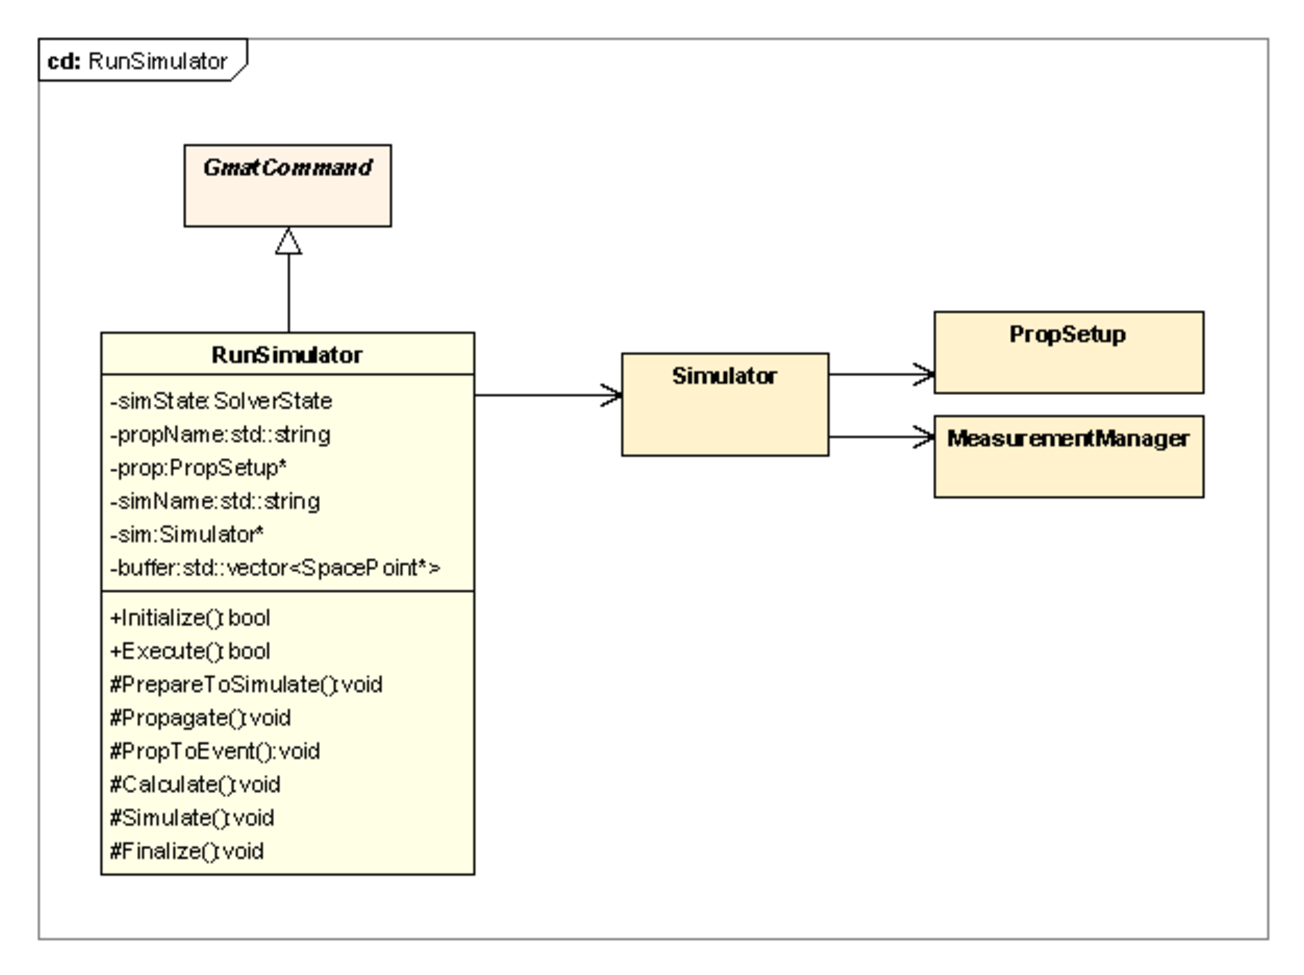
\includegraphics[scale=0.6]{Images/RunSimulator.eps}
% SimulatorOverview.png: 1201x516 pixel, 72dpi, 42.37x18.20 cm, bb=0 0 1201 516
\caption{\label{fig:RunSimulatorClass}The RunSimulator Class}
\end{center}
\end{figure}

\subsection{RunSimulator Members}

\paragraph{RunSimulator Attributes}

\begin{itemize}
\item \textbf{Gmat::SolverState simState}:  Tracks the state coming from the simulator's finite state machine so that appropriate actions can be triggered.
\item \textbf{std::string propName}:  Name of the PropSetup used to evolve the objects involved in the simulation.
\item \textbf{PropSetup *prop}:  A pointer to the simulator's copy of the configured PropSetup.
\item \textbf{std::string simName}:  The name of the simulator that implements the finite state machine.
\item \textbf{Simulator *sim}: A pointer to the simulator clone that is used with this command.
\item \textbf{std::vector<SpacePoint*> buffer}:  A local data buffer used to store copies of the simulation participants so that they can be restored later.
\end{itemize}

\paragraph{RunSimulator Methods}

\begin{itemize}
\item \textbf{virtual bool Initialize()}:  The method used to wire together all of components of the simulation that are available prior to execution of the Mission Control Sequence.
\item \textbf{virtual bool Execute()}:  The Mission Control Sequence entry point to the simulation.  This method makes calls to the AdvanceState() method on the simulator to drive the finite state machine.
\item \textbf{void PrepareToSimulate()}:  Method used to complete command initialization prior to execution of the finite state machine.  This method is triggered when the finite state machine is in the INITIALIZING state, prior to actual calls to the state machine.  The PropSetup completes initialization of its ODEModel and propagation state data during this call.
\item \textbf{void Propagate()}:  Propagates the components of the simulation when the finite state machine is in the PROPAGATING state.  This method queries the simulator for the desired time step (specified in seconds), and propagates by that duration to the next simulation epoch.  If the simulator specifies a zero time step, the command propagates by the natural time step of the propagator in the PropSetup.
\item \textbf{void PropToEvent()}:  Propagates the components of the simulation when the finite state machine is in the LOCATING state.  This method buffers the state data if necessary, queries the simulator for the desired time step (specified in seconds), and propagates by that duration to the next simulation epoch.  If the simulator specifies a zero time step, the command throws an exception and stops the simulation.
\item \textbf{void Calculate()}:  Method called when the finite state machine is in the CALCULATING state. This method is used to report status to the simulator text file.
\item \textbf{void Simulate()}:  Method called when the finite state machine is in the SIMULATING state. This method is used to report status to the simulator text file.
\item \textbf{void Finalize()}:  Cleans up the data structures used during the simulation, including the objects in the object buffer.  This method is triggered when the simulator is in the FINISHED state.
\end{itemize}
